It is important to reconstruct molecule from the \textit{asymmetric unit} (AU) preserving stoichiometric ratios. To handle this task program \textit{cif\_molecule}\cite{Grazulis2015} were developed as part of \textit{cod-tools} package.

\begin{tikzpicture}[>=latex]
    \node at ( 0,  0.5) {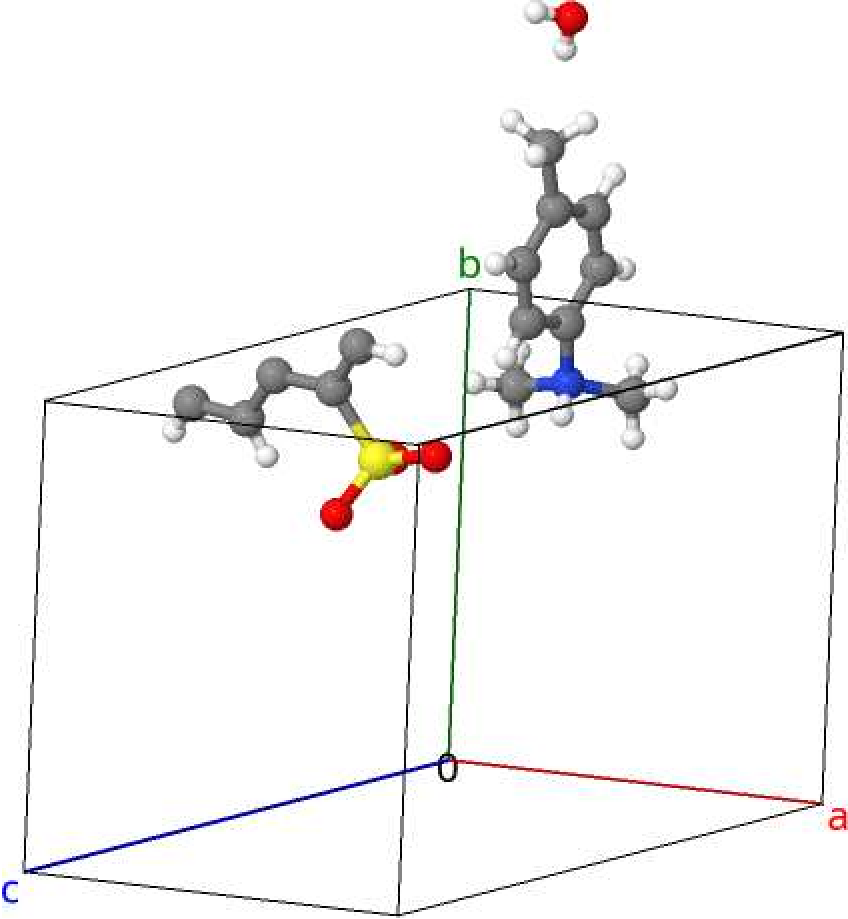
\includegraphics[scale=0.20]{pictures/2231955-crystal}};
    \node at ( 0, -2) {\small\itshape Asymmetric unit};

    \draw[->, ultra thick, rounded corners] ( 2,0) -- (5,0);
    \node at (4,1) {\small\texttt{cif\_molecule}};

    \node at (7, 0) {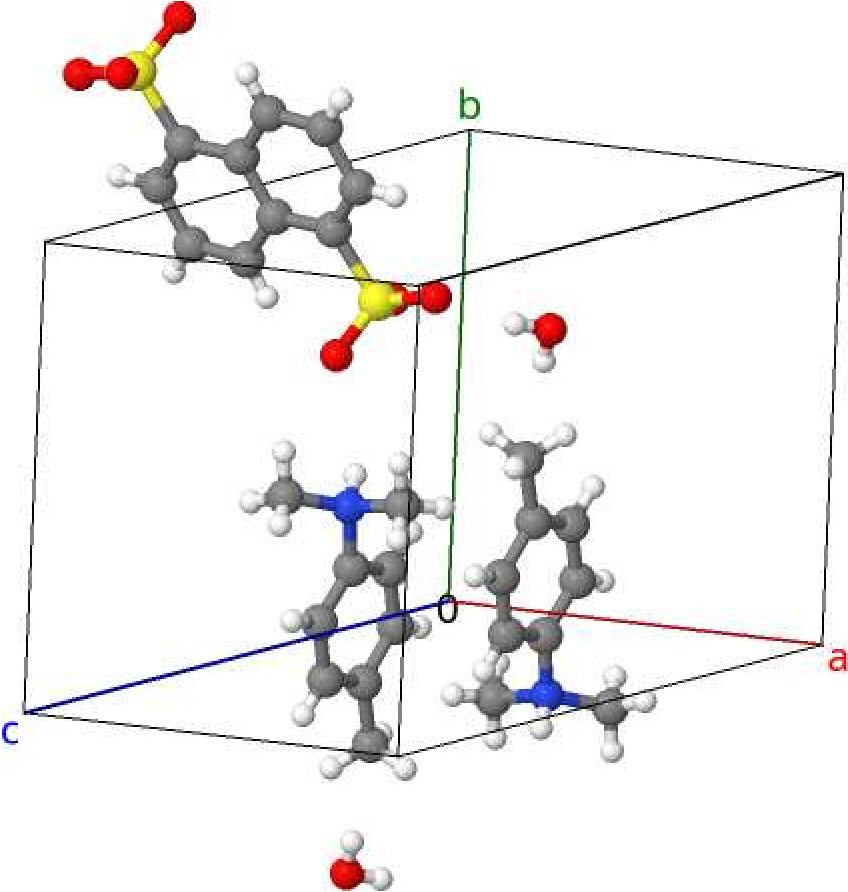
\includegraphics[scale=0.20]{pictures/2231955-chemical}};
    \node at (7,-2) {\small\itshape Stoichiometrically correct molecule};
\end{tikzpicture}

There are special kind of molecules, \textit{polymeric} molecules. Technical term is \textit{coordination polymers}, and there is a long history of problems with definitions \cite{Batten1998, Batten2012, Batten2013}. For our purposes we will consider \textit{polymer} an infinite molecule, which can be represented by an infinite repeated net. Infinite nature of \textit{polymers} presents problem on how to create a finite representation of such molecule.
There is an algorithm\cite{Chung1984} to solve this problem. It uses \textit{quotient graph} to describe all translational equivalent bonds and atoms. \textit{Quotient graph} algorithm uses notion of \textit{equivalence} to group \textit{equivalent} objects, in our case atoms are \textit{equivalent} if they have the same \textit{label} and \textit{symmetry operation} and algorithm will collect all \textit{equivalent} atoms into groups and add connections (edges) between them, we assign value to the edges.

Algorithm to create \textit{Labeled Quotient Graph} (LQG):

\begin{enumerate}\itemsep0pt
    \item Choose a coordinate system, select basis vectors.
    \item Assign initial labels to the original vertices $(0,0,0)$.
    \item If the net has an edge from point $P(m,n)$ to point $R(p,q)$ $\Rightarrow$ there is a directed edge in \textit{LQG} with label $(p-m, q-n)$ from $P$ to $R$.
\end{enumerate}

\begin{tikzpicture}[node distance=0.5cm, font=\small,>=Stealth]

\node[inner sep=0] (net) at (0,0)
    {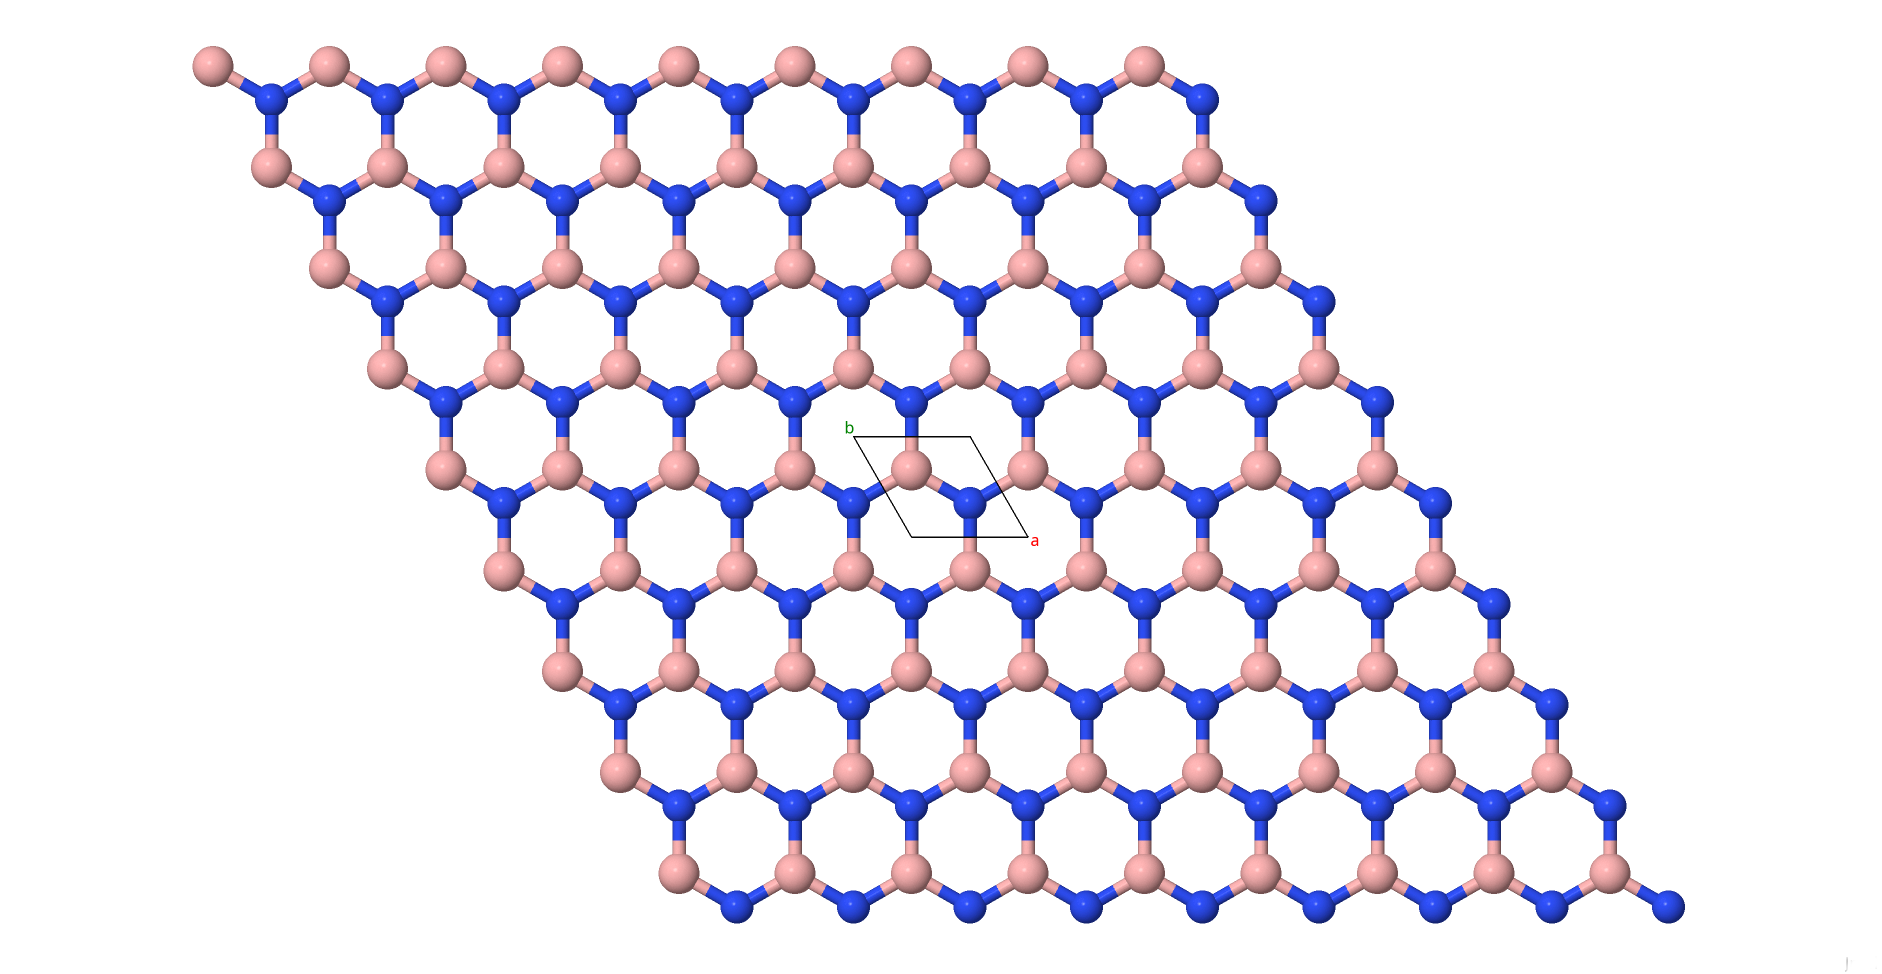
\includegraphics[width=0.4\textwidth]{pictures/9008997_cif_molecule2.png}};
    \node[below=1mm of net.south, font=\scriptsize\itshape] {Infinite net (COD ID \href{http://www.crystallography.net/cod/9008997.html}{\texttt{9008997}})};

\node[inner sep=0, right=5cm of net] (qg)
    {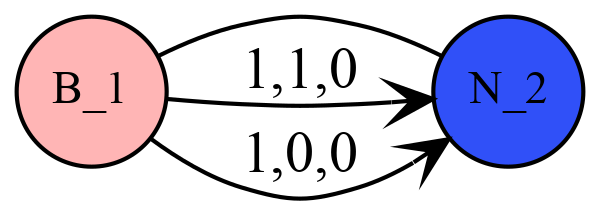
\includegraphics[width=0.25\textwidth]{pictures/9008997qg.png}};
    \node[below=1mm of qg.south, font=\scriptsize\itshape] {Labeled Quotient Graph (COD ID \href{svn://databases.crystallography.lt/quotient-graphs/trunk/outputs/polymers/default/9/00/89/9008997.dot}{\texttt{9008997}})};

\node[inner sep=0, right=3.5cm of net, below=2cm of $(net)!0.5!(qg)$] (tikzgraph){
    \begin{circuitikz}[scale=1]

        \draw (-1,26)--(2,26)--(3.5,24.25)--(0.5,24.25)--cycle;
        \draw (-4,26)--(-1,26)--(0.5,24.25)--(-2.5,24.25)--cycle;
        \draw (-2.5,27.75)--(0.5,27.75)--(2,26)--(-1,26)--cycle;

        \draw[short] (-1,24.75)--(0.5,25.5);
        \draw[short] (0.5,25.5)--(0.5,26.75);
        \draw[short] (0.5,25.5)--(2,24.75);

        \draw[fill={rgb,255:red,48; green,80; blue,248}]
            (0.5,26.75) circle(0.25cm) node[anchor=east, xshift=-10pt, yshift=-1pt, font=\scriptsize]{1,1,0};
        \draw[fill={rgb,255:red,48; green,80; blue,248}]
            (2,24.75) circle(0.25cm) node[anchor=east, xshift=-10pt, yshift=-1pt, font=\scriptsize]{1,0,0};
        \draw[fill={rgb,255:red,255; green,181; blue,181}]
            (0.5,25.5) circle(0.25cm) node[anchor=east, xshift=-10pt, yshift=-1pt, font=\scriptsize]{0,0,0};
        \draw[fill={rgb,255:red,48; green,80; blue,248}]
            (-1,24.75) circle(0.25cm) node[anchor=east, xshift=-10pt, yshift=-1pt, font=\scriptsize]{0,0,0};

        \coordinate(origin) at (-2.5,24.25);
        \coordinate(veca) at (3.5,24.25);
        \coordinate(vecb) at (-4,26);
        \draw[->,thick,red](origin)--(veca) node[midway,below,font=\scriptsize]{$\mathbf{a}$};
        \draw[->,thick,blue](origin)--(vecb) node[midway,left,font=\scriptsize]{$\mathbf{b}$};

    \end{circuitikz}
};
\node[below=1mm of tikzgraph.south, font=\scriptsize\itshape] 
    {Constructing Labeled Quotient Graph (LQG)};

\end{tikzpicture}

On the left you can see \textit{honycomb} net, at the center is a visual representation of the construction of \textit{LQG} and on the right is the result --- \textit{LQG}, vertex \textit{B\_1} represents all the \textit{Boron} atoms with symmetry operation 1, and vertex \textit{N\_2} represents all the \textit{Nitrogen} atoms with symmetry operation 2, 3 edges between these vertices represent all the possible translations that atoms can take, and can be used to reconstruct molecule.

\textit{LQG} algorithm was implemented in \textit{cif\_molecule} and released in \textit{cod-tools} release \textit{3.11.0}\cite{cod-tools}. \textit{cif\_molecule} were used on all the entries in the \textit{Crystallography Open Database} (COD)\cite{Grazulis2011}.

In addition to multiple tests that were already present, number of tests were added to the \textit{cif\_molecule}. But it is impossible to predict all the possible test cases. This potentially makes this algorithm a good target for creating formal specification that can be proved and improve confidence in the algorithm.
